% 
% Annual Cognitive Science Conference
% Sample LaTeX Paper -- Proceedings Format
% 

% Original : Ashwin Ram (ashwin@cc.gatech.edu)       04/01/1994
% Modified : Johanna Moore (jmoore@cs.pitt.edu)      03/17/1995
% Modified : David Noelle (noelle@ucsd.edu)          03/15/1996
% Modified : Pat Langley (langley@cs.stanford.edu)   01/26/1997
% Latex2e corrections by Ramin Charles Nakisa        01/28/1997 
% Modified : Tina Eliassi-Rad (eliassi@cs.wisc.edu)  01/31/1998
% Modified : Trisha Yannuzzi (trisha@ircs.upenn.edu) 12/28/1999 (in process)
% Modified : Mary Ellen Foster (M.E.Foster@ed.ac.uk) 12/11/2000
% Modified : Ken Forbus                              01/23/2004
% Modified : Eli M. Silk (esilk@pitt.edu)            05/24/2005
% Modified: Niels Taatgen (taatgen@cmu.edu)  10/24/2006

%% Change ``a4paper'' in the following line to ``letterpaper'' if you are
%% producing a letter-format document.






%%%% Remaining todos



\documentclass[10pt,letterpaper]{article}

\usepackage{cogsci}
\usepackage{pslatex}
\usepackage{apacite}
\usepackage{graphicx}
\usepackage{color}
\usepackage{amsmath}
\usepackage{multirow}
\usepackage{amssymb}
%\usepackage{url}
%\usepackage{hyperref}


 
\definecolor{Red}{RGB}{255,0,0}
\newcommand{\red}[1]{\textcolor{Red}{#1}}  


\title{ Lay theories of emotion in explaining behavior }
 
\author{{\large \bf Desmond C. Ong (dco@stanford.edu)} \\
{\large \bf Jamil Zaki (jzaki@stanford.edu))} \\
{\large \bf Noah Goodman (ngoodman@stanford.edu)} \\
  Department of Psychology, Stanford University, Stanford CA, USA 
}

\begin{document}

\maketitle

\begin{abstract}
Abstract

\textbf{Keywords:} 
Keywords
\end{abstract}

% Outline of paper

% More free-form
% Expt 1a) Emotions --> Actions
% Expt 1b) Generate cause of Actions. Coded into emotions, beliefs, situational factors, etc.

% More hypothesis driven
% Expt 2a) Actions / Expressions / Behavior, generate causes: Beliefs, Desire, Emotion, Situation factor
% Expt 2b) From 2a, for all actions/expressions/behavior, pick top b,d,e,s. Find endorsement rates of posterior using sliders.







%Talk about Malle's Cause vs. Reason. Intentional vs unintentional behavior

%evolutionary: emotions as strategic (e.g. Frank)

%Two hypotheses

%Folk Theory

One hypothesis is that in our lay theories of behavior, there are two distinct processes that result in two types of behavioral responses (see Figure \ref{ModelsOfBehaviorFig}a). The first of these processes is a rational decision making process in which an agent has a set of goals (``desires"), and a set of ideas on how to achieve those goals (often termed ``beliefs"). The agent then forms an intention to act upon his beliefs to achieve his desires, resulting in (intentional) action, as part of a ``belief-desire psychology" \cite{Dennett1989, Gopnik1997, Heider1958, Malle2011, Searle2001}. The second process, by contrast, relies on mere causality or ``impersonal causality" \cite{Heider1958}, and results in a second type of behavioral response. These behaviors could be caused by external situational factors, or as is often implicitly assumed by theories of folk psychology, the agent's emotions. Here, we make a distinction here between emotional expressions on one hand (e.g., crying), assumed to be caused only by emotions, and other unintentional behavior on the other (e.g. slipping on ice) that could be due to situational factors, and possibly emotions as well. Notably, in these theories of folk psychology, there is no place for emotions in the ``rational" decision making process that humans reason with when explaining the actions of others.

% Probably can say a bit more when I read those papers.

A second hypothesis is that emotions do play an important role in the formation and execution of intentional action. Figure \ref{ModelsOfBehaviorFig}b posits a lay theory in which emotions are factored into the intentional decision making process. This approach been incorporated into psychological \cite<e.g., >{Schwarz2000emotion}, economic \cite<e.g., >{Loewenstein2003affect}, and philosophical \cite<e.g., >{Zhu2002emotion} theories of behavior, but it is unclear how a theory of folk psychology incorporates emotions into the lay model of decision making \cite{Ong2015AffCog}. A third possibility that we must also consider is that the distinction between intentional action and emotional expressions in the lay theory is needlessly strong (Figure \ref{ModelsOfBehaviorFig}c), and that emotions, as well as beliefs and desires, impact an agent's intentional actions and emotional expressions. Indeed, emotional display rules (CITE XXX) and potential deceptive strategies (CITE XXX) do impact an agent's displayed emotional expressions, and might very well be an important factor in lay explanations of behavior. However, we (as have many theorists before us) reject the notion that all instances of emotional expressions are intentional, and hence should not be a subset of intentional action.

In this paper we provide some explorations of how emotions are incorporated into lay belief-desire psychology. We show that ...



\begin{figure}[htb!]
\begin{center}
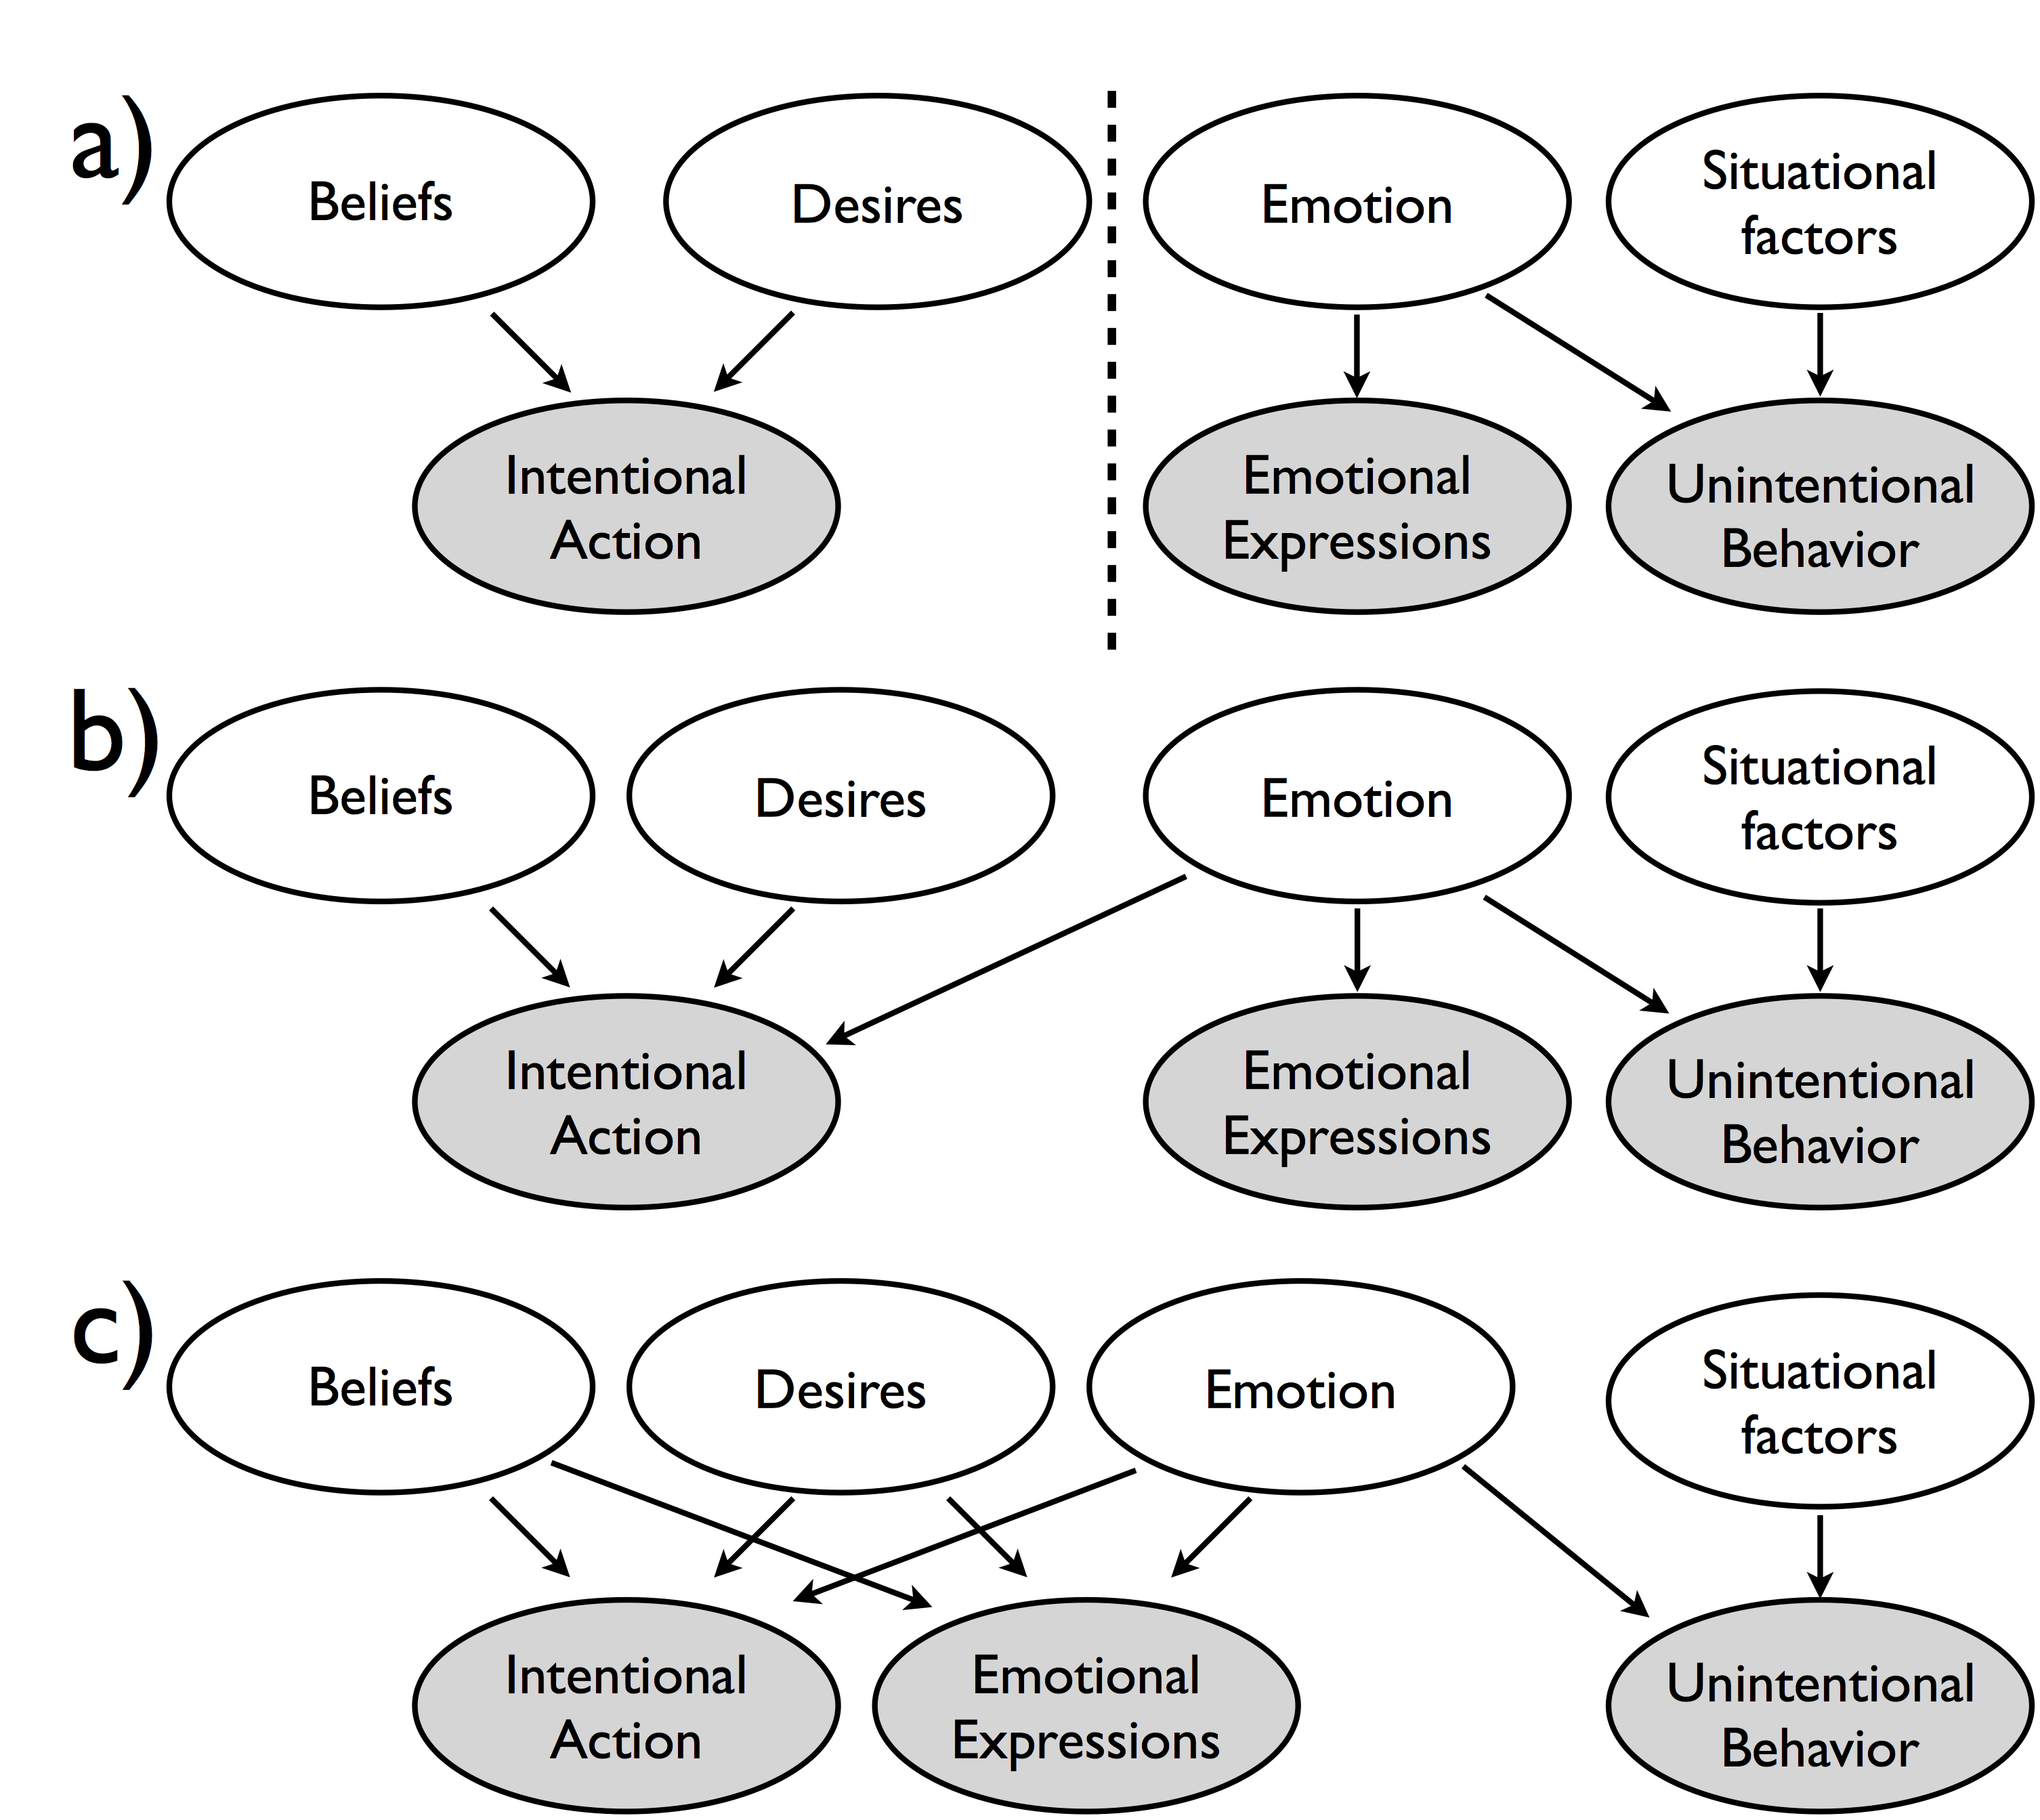
\includegraphics[width=1\columnwidth]{images/model1.png} 
\end{center}
\caption{ Possible lay theories of behavior. (a) There are two distinct types of behavioral responses; the rational decision-making process that goes from beliefs and desires to intentional action, and unintentional behavior and emotional expressions that are caused by situational factors and emotions. The latter process is governed by simple causality, without the need for an agent's intentionality. (b) Emotions do factor into the intentional decision making process, but there still exists emotional expressions and other unintentional behavior that are unaffected by beliefs and desires. (c) There is no distinction between intentional action and emotional expressions: both are affected by beliefs, desires and emotions.  }
\label{ModelsOfBehaviorFig}
\end{figure}


In order to test this, we elicited what types of behavior were most likely given 


%%%%


\section{Experiment 1}

	In Experiment 1\footnote{https://url/}, we tested if participants would X

% URL: http://web.stanford.edu/~dco/experiments/kidcf_bowling_v3/

\subsubsection{Participants and Procedures.} 
We recruited XXX adult participants ( ) through Amazon's Mechanical Turk (AMT).


%\begin{figure}[htb!]
%\begin{center}\includegraphics[width=1\columnwidth]{images/exptParadigm.png}\end{center}
%\caption{  }
%\label{ParadigmFig}
%\end{figure}



\subsubsection{Results.} 

\section{Experiment 2: }



\subsubsection{Results.} 





\section{Discussion}

Discuss

\section{Acknowledgments}

This work was supported in part by an A*STAR National Science Scholarship to DCO and by \red{XXX to NDG}.


\bibliographystyle{apacite}

\setlength{\bibleftmargin}{.125in}
\setlength{\bibindent}{-\bibleftmargin}

\bibliography{shakespeare_cogsci}





\end{document}
